\section{High Level PRNG Design and its Implication on DTLS Security} \label{LFSR}
We begin this section by reviewing how the 'default' PRNG (as provided by the CC2538) turns a seed into a stream of pseudo random numbers using a 16-bit LFSR (see CC2538 User's Guide\cite{CC2538Manual} Section 16.1). The polynomial that defines the feedback function is given as $x^{16} + x^{15} + x^{2} + 1$ which corresponds to the well known CRC16 scheme\cite{CRC}. When used as a PRNG (after it has been seeded), the input bit is simply set to zero. The CC2538 User's Guide\cite{CC2538Manual} gives clear instructions on how to use the LFSR: by setting specific control bits to 01, the LFSR performs 13 CRC16 operations and its content can be read out as a random number. 


% describes the PRNG design \begin{quote}
%The random-number generator is a 16-bit linear-feedback shift register (LFSR) with polynomial X 16 + X 15 +
%X 2 + 1 (that is, CRC16). It uses different levels of unrolling depending on the operation it performs. The basic version (no unrolling) is %shown in Figure 16-1 (\Cref{CRC16} in this paper). \end{quote}

%\begin{figure}[!t]
%\centering
%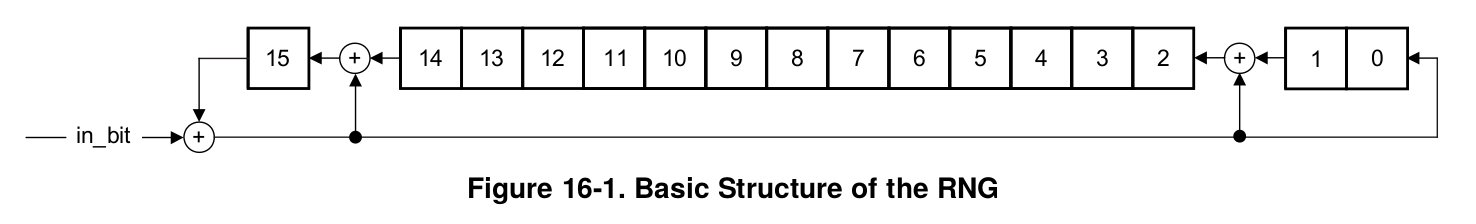
\includegraphics[width=2.5in]{fig/crc16.png}
%\caption{CRC16 LFSR, from CC2538 User's Guide}
%\label{CRC16}
%\end{figure}

%When used as a PRNG, the in\_bit in \Cref{CRC16} is constantly $0$. The Contiki driver calls the PRNG by: (Section 16.2.1in CC2538 User's Guide)
%\begin{quote}
%Another way to update the LFSR is to set the RCTRL bits in the SOC\_ADC\_ADCCON1 register to 01. This clocks the LFSR once (13x unrolling), and the RCTRL bits in the SOC\_ADC\_ADCCON1 register automatically clear when the operation completes.
%\end{quote}

%In another word, the LFSR is updated by performing 13 CRC16 operations in \Cref{CRC16} upon each RNG call. Since the CRC16 is deterministic and the register has only $16$ bits, the PRNG can be modelled as a Deterministic Finite Automaton (DFA) which made its output easily predictable as we will explain later in this section.

Formally, because there are only 16 bits in the LFSR, we can denote the universal set of its  possible values (or called states) $\mathbb{S}$ as:
\begin{equation} \label{PRNGState}
\mathbb{S} = \{ S_{i} | S_{i} \in \{2\}^{16}\}
\end{equation}
\Cref{PRNGState} implies that the LFSR can have no more than $|\mathbb{S}| = 2^{16} = 65536$ states.

We denote the LFSR update operation as:
\begin{equation}
F:\mathbb{S} \rightarrow \mathbb{S}
\end{equation}
where $F$ is $13$ times of CRC16 operation on the current state according to the manual.

Denote the 16 bits random seed sampled from the radio noise as $S^*$. The PRNG output can be formalised as:
\begin{equation}
	\begin{aligned}
	S_{0} &= S^* \\
	S_{i+1} &= F(S_{i})
	\end{aligned}
\end{equation}

Since $\mathbb{S}$ is finite and $F$ is deterministic, the random number stream is cyclic. The longest non-repetitive PRNG output sequence under seed $S^*$ can be represented as:
\begin{equation} \label{R*}
R_{S^*}= (F^0(S^{*}), F^{1}(S^{*}), ..., F^{n-2}(S^{*}), F^{n-1}(S^{*}))
\end{equation}
where $S^{*} = F^{0}(S^{*}) = F^{n}(S^{*})$. Each call to the PRNG effectively returns the first element in the sequence and updates it by one cyclic left rotation. Since the elements within $R_{S^*}$ are non-repetitive, we have $n \leq |\mathbb{S}|$ for any $R_{S^*}$, i.e. the cycle of PRNG output is at most $65536$ calls.

For a re-sampled seed $S^{*'}$ inside $R_{S^*}$, i.e. $S^{*'} = F^{k}(S^*)$ where $k \in \mathbb{Z}_n$, the corresponding sequence $R_{S^{*'}}$ is:
\begin{equation}\label{R*'}
	\begin{aligned}
	R_{S^{*'}} = &( F^{k}(S^*), F^{k+1}(S^{*}), ..., F^{n-1}(S^*), F^{0}(S^*), F^{1}(S^*),...,\\
	&F^{k-2}(S^{*}), F^{k-1}(S^{*}))
	\end{aligned}
\end{equation}

Observing \Cref{R*} and \Cref{R*'}, we can see $R_{S^*}$ is indeed $R_{S^{*'}}$ left rotated by $(n-k)$ times. This is equivalent to say that ${S^*}$ generates identical output as ${S^{*'}}$ with $(n-k)$ preceding calls. As a result, assume consecutive PRNG calls on $R_{S^*}$ returns a sequence of:
\begin{equation*}
(S_i, S_{i+1}, ..., S_{j})
\end{equation*}
Then the same sequence will eventually be replicated by calls on $R_{S^{*'}}$. This directly leads to the complete break of DTLS given the small space of $\mathbb{S}$, as we will explain in \Cref{BreakDTLS}.

This property also indicates that any seed not in $R_{S^*}$ generates a completely different sequence. By enumerating $\mathbb{S}$, we found there exists only four non-overlapping sequence for this CRC16 constructed PRNG, which are:
\begin{itemize}
	\item $R_{0x0001}$ with $n = 32767$.
	\item $R_{0x0003}$ with $n = 32767$.
	\item $R_{0x0000}$ with $n = 1$. ($F(0x0000) = 0x0000$)
	\item $R_{0x8003}$ with $n = 1$. ($F(0x8003) = 0x8003$)
\end{itemize}
Notice that $R_{0x0000}$ and $R_{0x8003}$ are excluded in the driver due to their monadic output according to the manual\cite{CC2538Manual}. The enumeration can be done on a CC2538 in less than a minute for such a small space of $65536$.

\subsection{Breaking DTLS} \label{BreakDTLS}
Contiki supports DTLS via an implementation called tinydtls\cite{tinydtls082}.  Two cipher suites, namely Pre-Shared Key\cite{rfc4279} (PSK) and ECDHE\_ECDSA\cite{rfc4492} are implemented by the latest available version (0.8.2) and the only supported curve is secp256r1\cite{secp256r1}. In this paper we only discuss ECDHE\_ECDSA. 

%As explained in \Cref{LFSR}, the CC2538 PRNG output is a predictable stream of cycle less than $2^{16}$ calls; therefore the possible key selection can be easily enumerated and leads to a complete break of cryptographic systems relies on its randomness.    

Unfortunately, tinydtls does not implement its own RNG; instead it loops the Contiki  API (random\_rand()) which is then implemented by the CC2538 built-in PRNG (see tinydlts/dtls\_prng.h) as we described in \Cref{LFSR}. As a result, the generated random numbers are from a very restricted set that is too small for any cryptographic use. This renders already any key generation vulnerable. A public Elliptic Curve (EC) key $Q$ is the scalar multiple $d$ of public base point $G$, i.e. $Q=[d]G$. Because $d$ can only take $2^{16}$ values, it is trivial to build a table for a specific curve and public base point that contains all pairs of $(d,Q)$. Consequently, upon observing a public EC key $Q$, one can use a simple table-lookup to deduce $d$. Due to the small entropy of CC2538 PRNG, such table contains only  $65536$ entries of $(d,Q)$ pairs which can be computed and stored on a laptop within a few minutes.

%When such RNG is used to generate an ECC key, the security notion is immediately broken as the random number is actually predictable as described in \Cref{LFSR}.
%\begin{figure}
%	\begin{algorithmic}[1]
%	\scriptsize
%	\REQUIRE Domain Parameter $T = (p, a, b, G, n, h)$ as specified by \cite{secp256r1}.
%	\STATE Randomly select $d \in [1, n-1]$.
%	\STATE Compute $Q = dG$.
%	\RETURN $(Q,d)$, where $Q$ is the public key and $d$ the secret key.
%	\end{algorithmic}
%	\caption{ECC Key Generation}
%	\label{KeyGen}
%\end{figure}

% \Cref{KeyGen} describes the ECC Key Generation. The RNG is involved in the selection of $d$. Since $T$ is public, an adversary can pre-compute the all possible public keys by enumerating all secret keys beginning in each position of $R_{0x0001}$ and $R_{0x0003}$. Upon observing a public key, the adversary can immediately look up its corresponding secret key in the pre-computed look up table. Since the look up table has only $65534$ entries, the pre-computation took less than 5 minutes on a laptop powered by i7-2620M. 
% 
Besides rendering key generation trivially insecure, one can further apply two trivial attacks  during a DTLS handshake. As before, these attacks work easily because of the poor randomness and the fact that popular EC schemes use public, standardised base points.

\paragraph{\textbf{ECDSA}}
	ECDSA\cite{ECDSA} is an authentication scheme that allows a party to authenticate a message. In DTLS, it is used to sign the server parameters (details in \cite{rfc3279}) during the handshake to provide server side authenticity. ECDSA requires a secret random number $k$ to generate a point on the curve $R$ via scalar multiplication of a base point. The x-coordinate $r$ of this point becomes part of the signature. Hence it can be observed by the adversary, who can recover $k$ by searching $r$ in the look up table of pre-computed points. He can then recover the secret signing key $d$ by computing:
	\begin{equation}
		\begin{aligned}
		e &= SHA-1(m) \\
		d &= r^{-1}(sk - e) \mod n
		\end{aligned}
	\end{equation}
	
%	\begin{figure}
%		\begin{algorithmic}[1]
%		\scriptsize
%		\REQUIRE Domain Parameter $T = (p, a, b, G, n, h)$, server key pair $(Q,d)$ and a message to be signed $m$.
%		\STATE Randomly select $k \in [1, n-1]]$.
%		\STATE Compute $kG = (x_1, y_1)$ and let $r = x_1 \mod n$.
%		\STATE Compute $e = SHA-1(m)$.
%		\STATE Compute $s = k^{-1}(e + dr) \mod n$.
%		\RETURN $(m,r,s)$ as the message-signature pair.
%		\end{algorithmic}
%		\caption{ECDSA Signing}
%		\label{ECDSA}
%	\end{figure}
	
\paragraph{\textbf{ECDHE}}
	ECDHE\cite{rfc4492} is a key exchange protocol that allows two party to derive a shared secret. In DTLS, ECDHE is performed at the end of DTLS handshake to derive a shared secret, which is then used to derive the symmetric session key for application data encryption. ECDHE essentially performs a Diffie-Hellman key agreement, i.e. one party computes $Q_A = [r_A]G$, the other party independently computes $Q_B = [r_B]G$; both parties exchange points, and so are able to derive  $Q_{AB} = [r_A][r_B]G = [r_A]{Q_B} = [r_B]{Q_A}$. Because $G$ is public, it is again possible to derive $r_A$ and $r_B$ by looking up $Q_A$ and $Q_B$  in the pre-computed table. Once these quantities are known to the adversaries, they can also compute $Q_{AB}$ and hence the session key.

%	\Cref{ECDHE} provides a brief description of ECDHE. The adversary can recover $r_A$ and $r_B$ by observing $Q_A$ and $Q_B$ that is being sent in the packets; hence computes $K$ to derive the symmetric key.
%	\begin{figure}
%		\begin{algorithmic}[1]
%		\scriptsize
%		\REQUIRE Domain Parameter $T = (p, a, b, G, n, h)$. Party $A$'s key pair $(Q_A, d_A)$ and party $B$'s key pair $(Q_B, d_B)$. 
%		\STATE $A$ randomly picks $r_A \in [0, n-1]$. 
%		\STATE $B$ randomly picks $r_B \in [0, n-1]$.
%		\STATE $A$ computes $Q_A = {r_A}G$ and sends $Q_A$ to $B$.
%		\STATE $B$ computes $Q_B = {r_B}G$ and sends $Q_B$ to $A$.
%		\STATE Both $A$ and $B$ computes $Q_{AB} = {r_A}{r_B}G = {r_A}{Q_B} = {r_B}{Q_A}$.
%		\RETURN Both $A$ and $B$ returns $K = Hash(Q_{AB})$ as the shared secret.
%		\end{algorithmic}
%		\caption{ECDHE}
%		\label{ECDHE}
%	\end{figure}

We have tested the attacks by sniffing two CC2538 nodes performing handshake using the example code provided in tinydtls. The secret keys have been successfully recovered using the look up table we generated.

\subsection{(P)RNG implementations in Contiki}\label{PRNGReflection}
%Stdlib implementation
Investigating (P)RNG implementations in other platforms supported by Contiki, we realised that most of them do not have dedicated PRNG implementations and by default wrap rand() in stdlib as their PRNG. We traced some of the open sourced stdlib implementations. For the majority of the libraries, i.e. stdlib for ARM\cite{ARMrand}, AVR\cite{AVRrand} and MSP430\cite{MSP430rand}, the rand() implementation can be abstracted as \Cref{rand}. The type of variable \textit{seed}  may vary on different platforms. The \textit{do\_rand()} function outputs a congruent of linear transformation of \textit{seed} and updates \textit{seed} by the output.
 
\begin{figure}
\lstinputlisting[breaklines=true,basicstyle=\scriptsize]{src/rand.c}
\caption{rand() implementations in stdlib}
\label{rand}
\end{figure}

It is clear that such design would also yield into a predictable random number stream with cycle no longer than the range of \textit{seed}, as the same \textit{seed} returns the same output. On the above platforms, the cycles are no longer than $2^{32}$, $2^{16}$ and $2^{16}$ calls respectively.

%Improvements (NIST 800-90A)
As a straightforward improvement, we suggest using more sophisticated PRNG implementation for cryptographic applications. \cite{NISTPRNG} has recommended several PRNG constructions based on approved hash functions and block ciphers. Specifically for CC2538, SHA-256 and AES have hardware coprocessor support and therefore can be considered candidates for implementing cryptographically secure PRNG according to \cite{NISTPRNG}.